%----------------------------------------------------------------------------
\appendix
%----------------------------------------------------------------------------
\chapter*{Appendices}\addcontentsline{toc}{chapter}{Appendices}\label{sect:Appendices}
\setcounter{chapter}{1}  % a fofejezet-szamlalo az angol ABC 1. betuje (A) lesz
\newcommand{\tab}[1]{\hspace{.1\textwidth}\rlap{#1}}


%----------------------------------------------------------------------------
\section{Modules and packages}
%----------------------------------------------------------------------------
\begin{figure}[!ht]
	\centering
	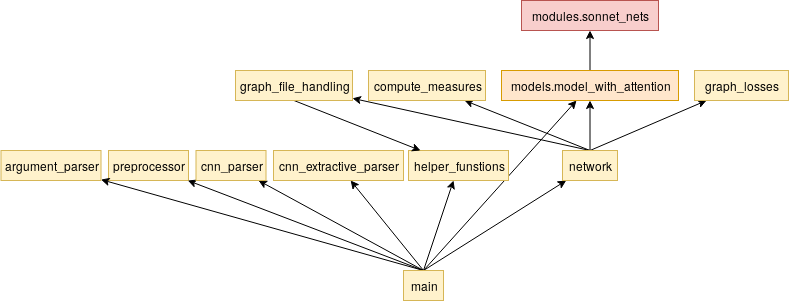
\includegraphics[width=150mm, keepaspectratio]{figures/packages_GraphTransformations.png}
	\caption{The most important modules and packages in the project}
	\label{fig:packages}
\end{figure}

\subsection{Functions and classes in each relevant module}

\begin{itemize}
	\item main.py
	\begin{itemize}
		\item predict function
		\item preprocess function
		\item test function
		\item train function
		\item visualize function
	\end{itemize}
	\item preprocessor.py
	\begin{itemize}
		\item dependency\_parse function
		\item process\_line function
		\item main function
	\end{itemize}
	\item cnn\_parser.py
	\begin{itemize}
		\item highlight\_to\_sentences function
		\item graph\_builder function
		\item main function
	\end{itemize}
	\item cnn\_extractive\_parser.py
	\begin{itemize}
		\item feature\_appender function
		\item article\_graph\_builder function
		\item main function
	\end{itemize}
	\item helper\_functions.py
	\begin{itemize}
		\item is\_valid\_graph function
		\item print\_graphs\_tuple function
		\item visualize\_graph function
		\item visualize\_original\_graph function
		\item visualize\_graph\_with\_colors function
	\end{itemize}
	\item network.py
	\begin{itemize}
		\item generate\_placeholder function
		\item train\_model function
		\item run\_session function
		\item train\_generator function
		\item predict function
		\item predict\_one\_graph function
		\item test function
	\end{itemize}
	\item compute\_measures.py
	\begin{itemize}
		\item compute\_accuracy function
		\item compute\_accuracy\_on\_nodes function
		\item compute\_accuracy\_ratio function
		\item compute\_one\_tp\_tn\_fp\_fn function
		\item compute\_tp\_tn\_fp\_fn function
		\item add\_tp\_tn\_fp\_fn function
		\item compute\_precision\_recall\_f1 function
	\end{itemize}
	\item graph\_losses.py
	\begin{itemize}
		\item regression\_loss function
		\item binary\_categorical\_loss function
		\item softmax\_loss function
		\item softmax\_loss\_on\_nodes function
	\end{itemize}
	\item graph\_file\_handling.py
	\begin{itemize}
		\item process\_line function
		\item load\_graphs function
		\item generate\_graph function
		\item get\_first\_batch\_graph\_dict function
		\item save\_predicted\_graphs function
	\end{itemize}
	\item models.model\_with\_attention.py
	\begin{itemize}
		\item Encoder class
		\item SimpleGraphAttention class
		\item GraphAttention class
	\end{itemize}
	\item modules.sonnet\_nets.py
	\begin{itemize}
		\item ActivatedLSTM class
		\item ActivatedLinear class
		\item NodeEmbedding class
		\item EdgeEmbedding class
		\item SimplifiedSelfAttention class
		\item GraphAttentionLayer class
	\end{itemize}
\end{itemize}

%----------------------------------------------------------------------------
\section{Class diagram}
%----------------------------------------------------------------------------
\begin{figure}[!ht]
	\centering
	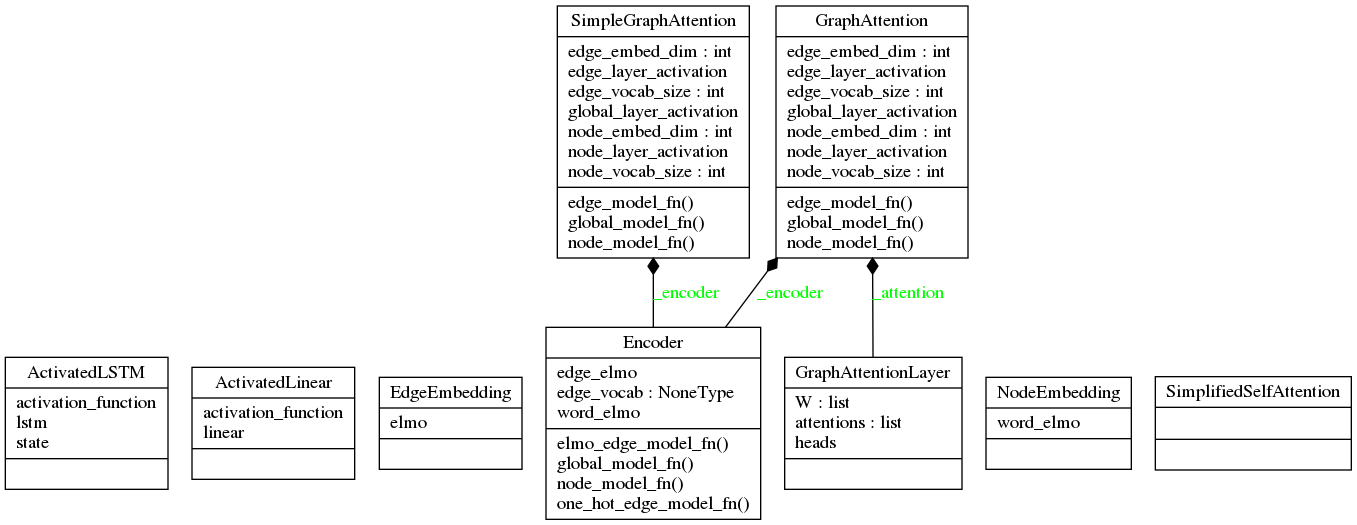
\includegraphics[width=150mm, keepaspectratio]{figures/classes_GraphTransformations.png}
	\caption{The classes in the project. The image was generated using \href{https://www.logilab.org/blogentry/6883}{Pyreverse}}
	\label{fig:classes}
\end{figure}


